\chapter[Metodologia]{Metodologia}
A metodologia escolhida para o desenvolvimento da plataforma será a metodologia ágil, a metodologia principal que vai será utilizada é o Kanban, porém, não será utilizada sua forma pura, e sim com algumas modificações, que atendem as necessidades do projeto. A escolha dessa metodologia se dá pelas seguintes características: o projeto será desenvolvido de maneira incremental, ou seja, ele poderá ser modificado no decorrer da implementação; a equipe consiste em apenas uma pessoa, o que descarta a possibilidade de utilizar o Scrum ou XP (\textit{Extreme Programming}); o escopo do projeto será dividido em tarefas, e a utilização do Kanban facilita no descobrimento de gargalos.

A metodologia Kanban surgiu no Japão com o TPS (Sistema Toyota de Produção) \cite{tps} para controlar a fabricação de automóveis e foi inserida no meio de desenvolvimento de software no ano de 2007. Kanban é um termo japonês para sinal visual e uma das grandes características dessa metodologia é evidenciar os problemas existentes no processo. 

A metodologia ágil surgiu no ano de 2001, com a reunião de especialistas em processos de desenvolvimento de software para discutir maneiras de melhorar o desempenho em projetos, com isso foi criado o Manifesto Ágil \cite{agil}. Uma das características das metodologias ágeis são sua capacidade de se adaptar a novos fatores durante o desenvolvimento do projeto, ao invés de tentar prever o que pode ou não acontecer.

\section{Análise de Ferramentas}
Nesta seção são feitos estudos sobre as ferramentas que serão utilizadas no desenvolvimento do projeto.
\subsection{Banco de Dados}
A ferramenta de banco de dados é responsável pelo armazenamento dos dados extraídos das fontes de dados.
\subsubsection*{Elasticsearch}
Elasticsearch é uma ferramenta \textit{open source}, desenvolvida pela Elastic\footnote[1]{\url{https://www.elastic.co/}}, de análise e busca REST capaz de resolver um grande número de casos. É a parte principal de Elastic Stack, servindo como um centro de armazenamento de dados \cite{elasticsearch}.

Elasticsearch suporta qualquer tipo de dado, além de agregar grande quantidades de dados para se ter uma visão melhor. Entre suas características as que mais se destacam são sua rapidez de busca, capacidade de detecção de falhas, múltiplos tipos de dados e suporte a múltiplas linguagens de programação.
\subsection{Frequência na Extração dos Dados}
Esta ferramente será responsável pela criação de uma rotina na hora de extrair os dados e atualizar o banco de dados.
\subsubsection*{Celery}
Celery é uma ferramenta \textit{open source} focada em operações em tempo real numa fila de tarefas assincronas baseadas na passagem de mensagens distribuidas, tambem oferece suporte a operações de agendamento \cite{celery}.

Celery possui funções que auxiliam a criação de rotinas, funcionando principalmente com Python\footnote[2]{\url{https://www.python.org/}}. Como Celery trabalha com a utilização de tarefas, podemos agendar seus funcionamentos utilizando \textit{cronjobs}\footnote[3]{\url{https://cron-job.org/en/}} para suas frequências.
\subsection{Visualização dos Dados}
Esta ferramenta será responsável por demonstrar os dados do banco de uma maneira mais intuitiva.
\subsubsection*{Kibana}
Kibana é um ferramenta \textit{open source}, desenvolvida pela Elastic, que permite a visualização dos dados guardados no Elasticsearch, possuindo diversas maneiras diferentes de disponibilização visual dos dados. É a parte de visualização do Elastic Stack, servindo como um centro de monitoramento \cite{kibana}.

\subsection{Criação de Containers}
Esta ferramente é responsável por dividir as partes da arquitetura em diferentes containers.
\subsubsection*{Docker}
Docker é uma ferramenta \textit{open source} que proveem containers de \textit{softwares} para o auxilios de desenvolvedores. Outras funcionalidades que são disponibilizadas são a integração com o desenvolvimento, suporte a multiplataformas e acesso a uma extensa biblioteca de servidores \cite{docker}.

\section{Arquitetura do Projeto}
A arquitetura do projeto é dividida em quatro partes: as fontes de dados, o extractor, o banco de indexação e a API RESTful. A ligação entre as partes e sua posição na arquitetura ficam evidenciado na figura \ref{image:arquitetura}.
\begin{figure} [H]
\centering
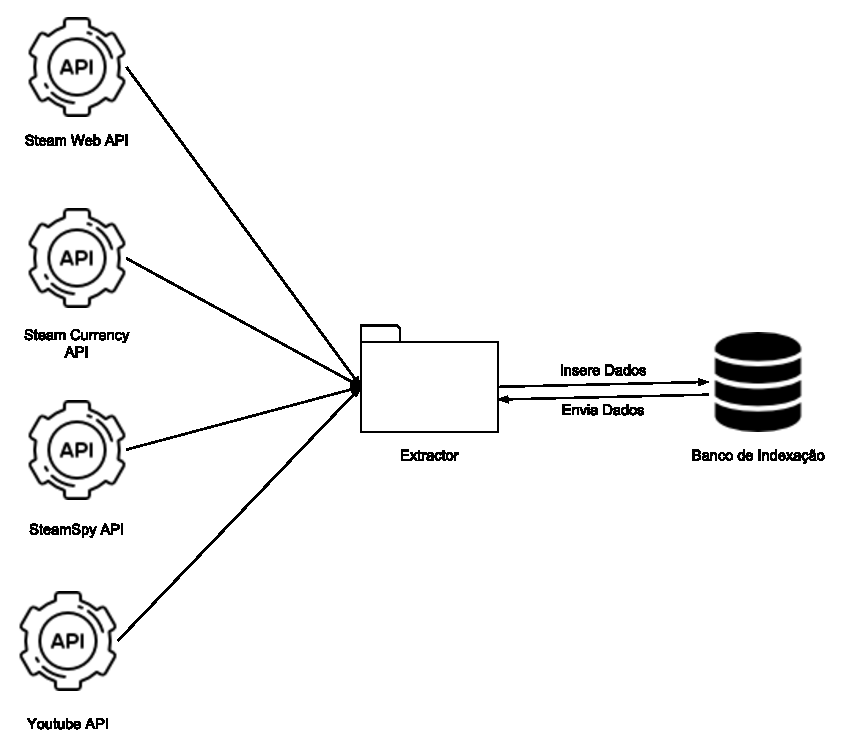
\includegraphics[scale=0.5]{figuras/arquiteturaProjeto.eps}
\caption{Arquitura Geral do Projeto}
\label{image:arquitetura}
\end{figure}
\textbf{Fonte de Dados} são locais onde se encontrar os dados que serão extraidos, manipulados e inseridos no banco de indexação, estes dados poderão vir de quaisquer fontes, sejam elas um banco de dados, de \textit{crawlers}, de APIs ou de arquivos locais.

\textbf{Banco de Indexação} é um banco de dados responsável por guardar os dados manipulados pelo Extractor. Como será utilizado o banco de jogos da Steam, o banco de indexação precisa suportar um grande número de dados e rapidez na atualização dos dados e na suas buscas.

\textbf{API RESTful} é a parte responsável por disponibilizar os dados do banco de indexação, sem que o usuário precise se conectar diretamente a ele. Como será desenvolvida um API, outros e quaisquers projetos poderão usufruir dela.
\subsection{Arquitetura Extractor}
A arquitetura do Extractor é composta de três classes principais e de dois arquivos e está representada na figura \ref{image:extractor}.
\begin{figure} [H]
\centering
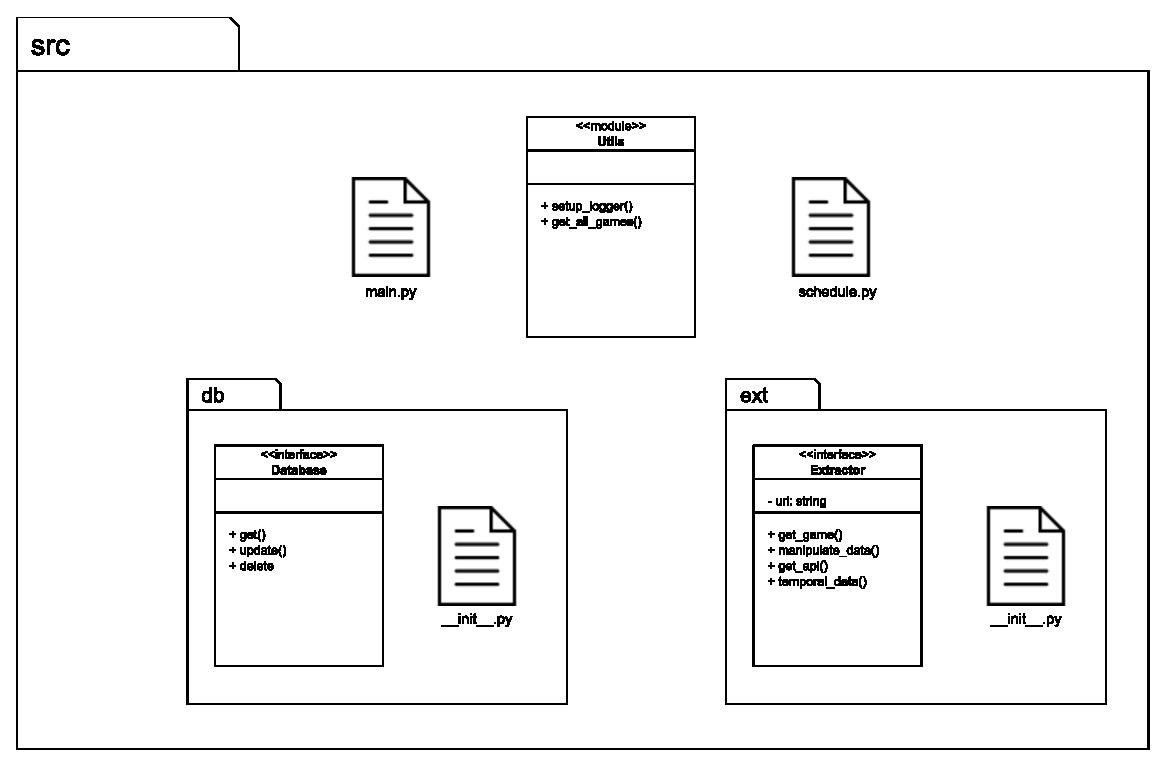
\includegraphics[scale=0.5]{figuras/arquiteturaExtractor.eps}
\caption{Arquitura do Extractor}
\label{image:extractor}
\end{figure}
A interface \textit{\textbf{Extractor}} deverá ser herdada por todos os plugins. Esta interface possui funções responsáveis por fazer requisições na API, extrair dados desta API e manipular estes dados, sejam eles estáticos ou temporais.

A interface \textit{\textbf{Database}} deverá ser herdada por todos os bancos de dados que possam a ser utilizado. Esta interface possui funções responsáveis por inserir/atualizar, deletar e mostrar os dados guardados pelo banco.

O módulo \textit{\textbf{Utils}} é responsável por implementar funções que não se encaixam em nenhuma classe do software. A princípio este módulo possui funções responsáveis por configurar os logs e extrair todos os jogos que possuem.

Os arquivos \textit{\textbf{Main}} e \textit{\textbf{Schedule}} são resposáveis por, respectivamente, fazer a primeira inserção no banco de dados e por manter um rotina de atualizações nos dados dos jogos.

\section{Extractor}
O Extractor é responsável pela extração, manipulação das informações das fontes de dados e também por inserir e atualizar o banco de dados. Como o Extractor lidará com dados que se modificam com o tempo, será preciso criar rotinas que lidarão com esses dados temporais. No escopo inicial serão utilizados quatro APIs.

A API \textit{\textbf{Steam WEB API}} é fornecida pela Steamworks\footnote[4]{\url{https://partner.steamgames.com}}, sendo assim é uma API oficial da Steam \cite{steam_api}. Ela possui métodos públicos e métodos privados. Os métodos públicos são abertos para qualquer usuário utilizá-los, já os métodos privados é necessário uma chave de desenvolvedor cedido pela própria Steamworks. Para acessar os dados da API é preciso um id, seja de usuário ou de jogo.

A API \textit{\textbf{Steam Store API}} é fornecida pela Steam. Ela disponibiliza informações sobre os jogos guardados no banco de dados da Steam. Para acessar estes dados é necessário o id do jogo na Steam, porém, também é possível passar filtros para pesquisas mais específicas.

A API \textit{\textbf{Steam Spy API}} é fornecida pelo Steam Spy. Ela também disponibiliza informações sobre os jogos, porém, dispõe-se de outras informações como o número de donos ou de avaliações positivas e negativas de um determinado jogo. Para acessar estes dados é necessário o id do jogo na Steam, porém, também é possível passar filtros para pesquisas mais específicas

A API \textit{\textbf{Youtube API}} é fornecida pelo Google Developers\footnote[5]{\url{https://developers.google.com/}}, sendo assim a API oficial do Youtube. Ela dispõe de informações sobre cada vídeo como os números de likes, dislikes e visualizações. Para extrair os dados de cada vídeo é necessário conseguir a lista dos 20 vídeos mais relevantes de um jogo, após isso com o id dos vídeos extrair suas informações.

A relação entre os dados que serão extraídos e de qual API será utilizado esta representado na tabela \ref{table:dados}.
\begin{table} [H]
\centering
\scalebox{0.7}{
\begin{tabular}{|c|c|c|c|c|}
\hline &\textit{\textbf{Steam WEB API}}&\textit{\textbf{Steam Spy API}}&\textit{\textbf{Steam Store API}}&\textit{\textbf{Youtube API}} \\
\hline Nome&&&\cellcolor{green}& \\
\hline Descrição&&&\cellcolor{green}& \\
\hline Imagem \textit{Header}&&&\cellcolor{green}& \\
\hline Imagem \textit{Background}&&&\cellcolor{green}& \\
\hline \textit{Website}&&&\cellcolor{green}& \\
\hline Data Lançamento&&&\cellcolor{green}& \\
\hline Steam Id&&&\cellcolor{green}& \\
\hline Metacritic \textit{Score}&&&\cellcolor{green}& \\
\hline Avaliação Positiva&&\cellcolor{green}&& \\
\hline Avaliação Negatica&&\cellcolor{green}&& \\
\hline Média de Horas&&\cellcolor{blue}&& \\
\hline Donos&&\cellcolor{blue}&& \\
\hline Jogadores Online&\cellcolor{blue}&&& \\
\hline Visualizações&&&&\cellcolor{blue} \\
\hline \textit{Likes}&&&&\cellcolor{blue} \\
\hline \textit{Dislikes}&&&&\cellcolor{blue} \\
\hline \textit{Userscore}&&\cellcolor{blue}&& \\
\hline Gêneros&&&\cellcolor{green}& \\
\hline Categorias&&\cellcolor{green}&& \\
\hline Linguagens&&\cellcolor{green}&& \\
\hline \textit{Screenshots}&&&\cellcolor{green}& \\
\hline Desenvolvedoras&&&\cellcolor{green}& \\
\hline Publicadoras&&&\cellcolor{green}& \\
\hline Plataformas&&&\cellcolor{green}& \\
\hline Preço&&&\cellcolor{blue}& \\
\hline \multicolumn{5}{|c|}{Legendas} \\
\hline \multicolumn{4}{|l|}{Dados Estáticos}&\cellcolor{green} \\
\hline \multicolumn{4}{|l|}{Dados Temporais}&\cellcolor{blue} \\
\hline
\end{tabular}}
\caption{Dados x APIs}
\label{table:dados}
\end{table}
\subsection{Dados Temporais}
Dados temporais são aqueles dados que serão atualizados de acordo com alguma frequência. Como serão guardados seus valores no decorrer do tempo, será possível comporar o mesmo dado de um jogo num determinado espaço de tempo, podendo assim extrair mais informações e ocasionalmente mais métricas. A frequência que estes dados serão atualizado estão representado na tabela \ref{table:frequencia}.
\begin{table} [H]
\centering
\begin{tabular} {c|c}
\textbf{Tipo do Dado}&\textbf{Frequência} \\
\hline Média de Horas&1 vez por semana \\
\hline Donos&1 vez por semana \\
\hline Jogadores Online&1 vez por dia \\
\hline Visualizações&1 vez por dia \\
\hline \textit{Likes}&1 vez por dia \\
\hline \textit{Dislikes}&1 vez por dia \\
\hline \textit{Userscore}&1 vez por semana \\
\hline Preço&1 vez por semana \\
\hline 
\end{tabular}
\caption{Dados x Frequência}
\label{table:frequencia}
\end{table}

Outro função que será chamanda numa determinada frequência será a inserção de novos jogos no banco de dados, pois novos jogos são lançandos a cada dia. Para não causar uma sobrecarga no Celery, a inserção de novos jogos ocorrerão uma vez por semana.
% \section{API de Consumo}
% A API de consumo será responsável por consumir o banco de indexação, e partir dos dados gerar \textit{end points} REST para que qualquer aplicação possa utilizá-la. A API deverá atualizar seus \textit{end points} com a mesma frequência com o qual o software de extração atualiza o banco de indexação.

% A API possuirá dois \textit{end points}: uma para gerar informações sobres os jogos no banco de indexação e outro para gerar \textit{rankings} para um determinado perfil.

% O \textit{end point} de informações dos jogos poderá receber vários filtros, sendo os mais comuns: pegar todos os jogos disponíveis no banco de indexação, pegar todos os jogos de um ou mais gêneros, pegar todos os jogos com uma ou mais determinadas categorias. Os \textit{end points} mais comuns são:
% \begin{itemize}
% 	\item \textit{https://api/games/all}
% 	\item \textit{https://api/games/genre=action}
% 	\item \textit{https://api/games/categories=atmospheric}
% \end{itemize}
% O \textit{end points} de \textit{rankings} gerarão \textit{rankings} a partir de determinados filtros, sendo os mais comuns: gerar um \textit{rankings} pelos jogos mais jogados naquele momento, gerar um \textit{rankings} com os jogos que possui as maiores porcentagens de avaliações positivas. A API também deverá gerar qualquer ranking com os filtros de gêneros e categorias, ou seja, deve-se gerar um ranking qualquer para um determinado perfil de jogo. Os \textit{end points} mais comuns são:
% \begin{itemize}
% 	\item \textit{https://api/rankings/all}
% 	\item \textit{https://api/rankings/current}
% 	\item \textit{https://api/rankings/avaliation}
% \end{itemize}